\subsection{Theoretische Grundlagen}

\subsubsection{Überblick}
In der Rastertunnelmikroskopie wird die Oberfläche von Festkörpern untersucht. 
Dabei wird der quantenmechanische Tunneleffekt ausgenutzt, der einen minimalen 
Stromfluss dort erlaubt, wo klassisch die Potentialbarriere zu hoch wäre. 
Die Wahrscheinlichkeit, dass ein Elektron durch die Barriere ”tunnelt”, 
hängt stark von der Breite derselben ab – daher kann der Tunnelstrom als 
Messgröße für die Entfernung zwischen Spitze und Oberfläche benutzt werden. 
Mit Hilfe des entsprechenden theoretischen Zusammenhanges und Modellen aus 
der Festkörperphysik können so Bilder von der Oberfläche gemacht werden und 
Parameter wie die Gitterkonstante berechnet werden. Untersucht werden in 
diesem Versuch die Oberflächen von Graphit, einer mit Gold beschichteten 
Struktur und des Halbleiters $\mathrm{MoS_2}$. 


\subsubsection{Grundlagen der Festkörperphysik}
Wir gehen in unserer Beschreibung der untersuchten Metalle und Halbleiter 
vom Bändermodell aus. Durch die gegenseitige Beeinflussung der Atome im Gitter
werden die im Einzelatom noch stark voneinander abgetrennten Energie-Eigenzustände
der Elektronen aufgespalten und folgen so dicht aufeinander, dass Elektronen 
sehr leicht zwischen den einzelnen Zuständen wechseln können. Die atomaren
Energieniveaus bleiben jedoch zum Großteil soweit getrennt, dass klar definierte
"Bänder" entstehen. Das für $T = 0\deg K$ äußere Energieband ist das Valenzband.
Die zur chemischen Bindung beitragenden Elektronen gehören genau diesem Band an 
(Valenz = Bindung, Valenzelektronen). Das über dem Valenzband liegende Band wird 
als Leitungsband bezeichnet. Elektronen im Leitungsband sind räumlich nicht mehr 
gebunden, da sich die Orbitale der jeweiligen Atome überlagern – diese Elektronen 
können daher leicht Energie eines elektrischen Feldes aufnehmen und sich in dem 
Gitter bewegen. \\


\subsection{Grundlagen der Festkörperoberflächen}
Bei der Beobachtung der Oberflächen von Festkörpern sind die Modelle unendlich 
ausgedehnter Kristallgitter nur teilweise zu verwerten, da an den Oberflächen 
oft zusätzliche Effekte auftreten. Eine Kategorisierung wird von Henzler und 
Göpel \cite{henzler1991oberflachenphysik} gegeben (Abb.: \ref{fig:oberflaeche}).
Grundsätzlich kann es Abweichungen der regelmäßigen, dreidimensionalen 
Oberflächenstruktur in null, ein, zwei oder drei Dimensionen geben. Letztere 
sind Abweichungen der unterliegenden Baustruktur, die zum Teil eine Mosaikstruktur 
bilden, die sich auch auf größere Skalen erstrecken. Zweidimensionale Strukturen 
tauchen als großflächige Überstrukturen oder kleinere Facetten auf. 

Zur mathematischen Beschreibung werden die Gittervektoren aus dem Ortsraum benutzt, 
die in der Oberfläche liegen. Ausreichend sind meistens jene aus der obersten 
Atomschicht. Die Atome befinden sich dann an den Positionen 
\begin{equation}
    \mathbf{r} = m_1 \mathbf{a_1} + m_2 \mathbf{a_2},
\end{equation}
wobei nach Konvention $|\mathbf{a_1}| \le |\mathbf{a_2}|$ und 
$\gamma = \angle (\mathbf{a_1}, \mathbf{a_2}) > 90 \deg$ der Winkel zwischen den 
beiden Vektoren ist. Da die Atom in einer Ebene liegen, ist die Anzahl möglicher 
Anordnungen, die sog. Bravais-Netze, deutlich kleiner als für einen 3D-Kristall. 
Es gibt genau fünf, wie in Abb.~\ref{fig:Bravais} gezeigt 
\cite{henzler1991oberflachenphysik}.
Zur vollständigen Beschreibung fehlen dann allerdings noch die Angaben zur Lage 
der Oberflächenatome relativ zur darunter befindlichen Basis. 

Zur Beschreibung der Oberfläche wird zuerst die ideale Oberfläche angenommen, 
die sich aus dem darunter liegenden Kristallgitter ergäbe, und deren Vektoren mit
$|\mathbf{a_1}| \le |\mathbf{a_2}|$ bezeichnet werden. Die tatsächle Struktur, 
soweit periodisch, kann dann als Verhältnisse $\frac{\mathbf{a_1}}{\mathbf{b_1}}$, 
$\frac{\mathbf{a_1}}{\mathbf{b_1}}$ und Winkel zwischen Basis und Oberfläche angegeben 
werden. Zusammen mit der Millerschen Schreibweise für die Kristallfläche der Basis 
ergibt sich so eine kompakte Schreibweise, z.~B. 
$\mathrm{Si}(111)(\sqrt{3} \times \sqrt{3}) \mathrm{R} 30 \deg$. 
Ist diese Schreibweise ungeeignet aufgrund fehlender Symmetrien, so kann eine 
Matrixschreibweise benutzt werden. Sind die Einträge ganze Zahlen, so liegen die 
Atome der Oberfläche direkt auf der Basis. Bei rationalen Zahlen gibt es auch 
zwischen den Basisatomen Oberflächenatome, während bei irrationalen Zahlen die 
Oberfläche quasi unabhänging von der Basis gesehen werden muss. Sie wird dann auch 
als inkommensurabel bezeichnet. \cite{henzler1991oberflachenphysik}

\begin{figure}
    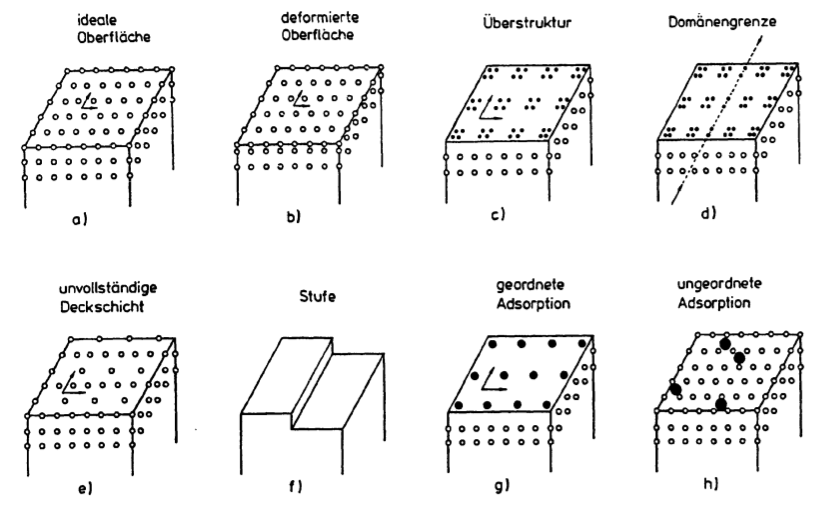
\includegraphics[width=1.0\textwidth]{pics/oberflaechenstruktur}
    \caption{Die ideale Oberfläche und einige mögliche Oberflächenstrukturen, 
aus \cite{henzler1991oberflachenphysik} }
    \label{fig:oberflaeche}
\end{figure} 
\begin{figure}
    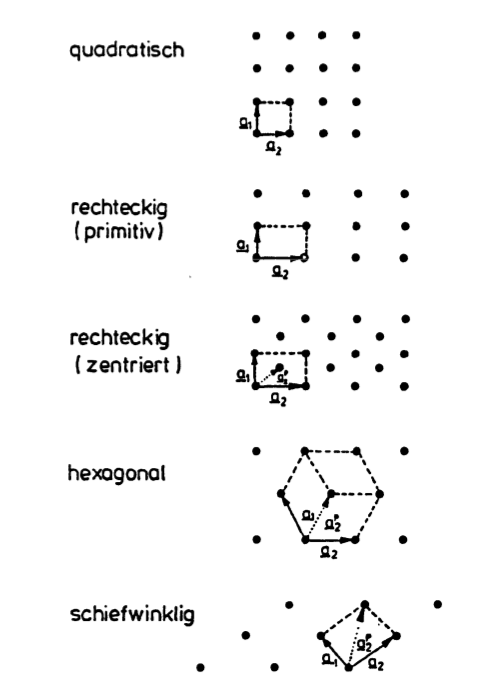
\includegraphics[width=0.5\textwidth]{pics/Bravais}
    \caption{Bravais-Gitter zur Oberflächenstrukturbeschreibung. Die kleinstmöglichen
Zellen sind in den unteren drei Gittern mit $\underline{a}_2^p$ beschriftet. 
Aus \cite{henzler1991oberflachenphysik} }
    \label{fig:Bravais}
\end{figure} 


\subsection{Struktur von Graphit, Gold und $\mathrm{MoS_2}$}
Die Kristallstruktur von Graphit zeichnet sich vor allem durch seine Schichtenstruktur 
aus. Die Kohlenstoffatome sind in den aus kovalent gebundenen Sechsecken bestehenden 
Basalebenen oder Graphenschichten deutlich fester aneinander gebunden (4.3 eV), als 
an solche aus benachbarten Schichten (0.07 eV). Daher ist Graphit entlang dieser Linien 
sowohl mechnisch deutlich stabiler als auch sehr viel leitfähiger (für Wärme und 
elektrischen Strom). Graphit tritt nicht nur in zueinander korrlierten Schichten auf, 
sondern auch unkorrliert (sog. turbostratischer Kohlenstoff). Die hier untersuchte Form 
ist jedoch regelmäßig - die Winkelabweichung für das verwendete HOPG (highlz orientated 
pzrolztic graphite) beträgt weniger als $1 \deg$. Es liegen in der Schichtung jedoch 
nicht alle Atome übereinander, sondern lediglich jedes zweite aus jedem Sechseck (siehe 
Abb.~\ref{fig:graphite}). Dadurch kommt es an der Oberfläche zu einem oft beobachteten 
Effekt: Anstatt sämtliche Atome der Sechsecke zu beobachten, taucht nur die Hälfte auf 
den STM-Bildern auf. Erklärt wird das dadurch, dass die Elektronendichte in der 
Fermienergie für Atome mit Nachbarn darunter höher liegt als bei solchen ohne
\cite{zeinalipour2008new}. Selloni~et~al.~\cite{Sellino1985} berechneten den Abstand 
der Atome mit bzw. ohne direkten Nachbarn in der Schicht darunter mit $0.15 \AA$. 

\begin{figure}
    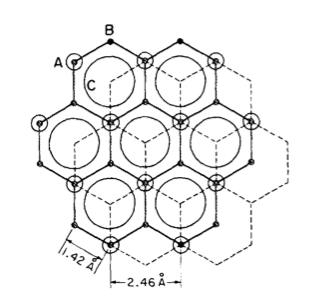
\includegraphics[width=1.0\textwidth]{pics/graphite}
    \caption{Hexagonale Oberflächenstruktur von Graphit, aus \cite{park1986tunneling}}
    \label{fig:graphite}
\end{figure} 

